\externaldocument{Introduction.tex}
\externaldocument{Experimental_Apparatus.tex}
\externaldocument{Results.tex}
\externaldocument{Analysis.tex}
\externaldocument{EIC_Jets.tex}
\externaldocument{Checks_and_Systematics.tex}
% \externaldocument{Discussion.tex}

\section{Integrated Statistical Uncertainty on Fragmentation Function Ratio}
For the purpose of giving a single number to quantify how similar pp and \pPb~ fragmentation functions are, an integrated statistical uncertainty on the ratio of the two was calculated \footnote{The p-value calculated from the two distributions only indicates that the null hypothesis, pp and \pPb~ are the same, cannot be rejected}. First, the fragmentation function in pp was integrated, and the statistical errors were added in quadrature. The summed statistical uncertainty was then divided by this integral to obtain the relative uncertainty. The same was done for the \pPb~ fragmentation function. Then, the two relative uncertainties were added in quadrature and the ratio of the integrals was taken. This is shown in equation~\ref{eq:fragErrorRatio} below,

\begin{equation}\label{eq:fragErrorRatio}
  \begin{split}
    I &= \sum_i y_i\cdot z_i \\
    \delta_\mathrm{abs.} &= \delta_0 \oplus \delta_1 \oplus ...\delta_n\\
    \delta_\mathrm{rel} &= \frac{\delta_\mathrm{abs.}}{I},\\
  \end{split}
\end{equation}{}
where $I$ is the integral of the fragmentation function, $y_i$ is the conditional yield of associated hadrons in \zt~ bin i, and $z_i$ is the width of \zt~ bin i. Additionally, $n$ is the number of \zt~ bins, and $\delta_i$ is the statistical uncertainty of the $i_\mathrm{th}$ \zt~ bin. $\delta_\mathrm{rel}$ is the relative statistical error on the fragmentation function. Taking the ratio of the integrals and summing the uncertainties from pp and \pPb~ in quadrature:

\begin{equation}
  \delta_\mathrm{ratio} = \frac{I_\mathrm{p-Pb}}{I_\mathrm{pp}}\cdot (\delta_\mathrm{rel,pp} \oplus \delta_\mathrm{rel,p-Pb}),
\end{equation}

yields a total integrated statistical uncertainty on the ratio, $\delta_\mathrm{ratio}$ of 13\%. Thus, modifications to the fragmentation function in \pPb~are constrained to be less than 13\%. This measurement probes the transverse momentum fraction range of {$x_{\mathrm{T}} = 2\pt/\sqrt{s_{\mathrm{NN}}}\ = $ 0.005--0.016}. This $x_{\mathrm{T}}$ range is similar to RHIC measurements at forward rapidity~\cite{Adare:2011sc}.

This measurement marks the first study of photon-tagged fragmentation in \pPb~collisions at the LHC. A precise measurement of $Q^2$ in heavy ion collisions is not possible without reconstructing all particles in the event. Nonetheless, among the LHC experiments, ALICE is uniquely configured to measure low-\pt~charged particles. In the context of jet constituents and total jet \pt, ALICE is capable of measuring hard scatterings with a lower $Q^{2}$ than other LHC experiments. Previous data have shown that, at sufficiently high $Q^2$ there is no fundamental difference in the scattering off a nucleon or off a nucleus \cite{epps16:2017,ALTARELLI1977298}. Thus, the kinematic range of this study is of particular interest for studying cold nuclear matter effects, as they are expected to be largest at lower $Q^{2}$ \cite{epps16:2017}. 

The agreement between pp and \pPb~in this kinematic range constrains modifications to the parton fragmentation function to be less than the integrated uncertainty of 13\% on the \pPb/pp ratio for $ 0.005 < x_{\mathrm{T}} < 0.016$, and partons with approximately $12 < \pt < 40$\GeVc. This region in $x_\mathrm{T}$ is particularly important to keep in mind when comparing the measurement to CNM calculations and nPDFs.

\section{Insensitivity to Parton Distribution Function}
\label{sec:insensitivity}
\ref{sec:FF} detailed the factorization of the hadronic cross section into the product of the parton distribution function (PDF) and the fragmentation function (FF). One of the goals of this study is to better understand the modification of the fragmentation function in \pPb~collisions. A very important question for the fragmentation function in \pPb~collisions compared to pp collisions is: How do we know if modifications to the observed $\gamma$-tagged associated yields are due to the PDF, and not in fact modifications to the fragmentation function?

To answer this question, the prompt photon and hadronic cross sections need to be understood, particularly the nPDFs present in both cross sections. Because the main observable is the conditional yield of hadrons per photon, modifications to the cross production cross sections cancel. Coupled with the fact that photons are not otherwise be affected by nuclear effects \cite{\cite{Chatrchyan2012}, this measurement helps elucidate the impact of cold nuclear modification on the parton fragmentation function. Eq.~\ref{eq:photon_cross} shows the factorized inclusive cross section of prompt photons in heavy ion collisions adapted from \cite{Catani2002}, and Eq.~\ref{eq:hadron_cross} shows the hadron cross section (shown in section \ref{sec:FF}, but displayed here again for convenience):


\begin{equation}
  \sigma^{A+B\rightarrow\gamma+X} = \int dx_a dx_b dz \sum_{a,b}f_{a}(x_a)f_{b}(x_b) \hat{\sigma}^{a+b\rightarrow\gamma+X'}
\end{equation}
\label{eq:photon_cross}

\begin{equation}
  \sigma^h= \sum_{a,b,c} \int dx_a dx_b dz f_a(x_a) f_b(x_b) d\hat{\sigma}(p_a,p_b,p_c) D_c^h(z).
  \label{eq:hadron_cross}
\end{equation}

The sum is over the flavor of incoming partons $a$ and  $b$ with $f_{a},(x_a)$ and  $f_{b},(x_b)$ being the nPDFs of the incoming partons. The nPDF is simply the nuclear parton distribution function and applies to nucleons that make up a larger nucleus, in this case lead. In Eq.~\ref{eq:photon_cross}, $\hat{\sigma}^{a+b\rightarrow\gamma+X'}$ is the prompt photon production cross section in parton-parton collisions, and can be further factorized into $\sigma_\mathrm{dir}$ and $\sigma_\mathrm{frag}$ as done in \cite{williams2018}. The hadron cross section sums over an additional parton flavor $c$ to include the outgoing parton's fragmentation function, $D_c^h(z)$, that produces the final state hadrons. It is important to note that Eq.~\ref{eq:hadron_cross} is not the inclusive cross section of charged hadrons (such a cross section would include significant contribution from the underlying event, which is subtracted in this measurement), but instead corresponds to hadrons produced from the scattered parton. What's important about these two equations is that the underlying form of the nPDFs in both equations, $f_{a}(x_a)$ and $f_{b}(x_b)$, is identical in this factorization scheme. 

Ignoring detector effects, the measured yield of prompt photons should be directly proportional to the product of Luminosity and the cross section:

\begin{equation}
  Y = \mathcal{L}\times\sigma
\end{equation}

The same logic applies to the yield of charged hadrons. The observable in this study, the conditional yield of charged hadrons associated with isolated prompt photons, is essentially the ratio of measured yields, and by extension the ratio of cross-sections described in Eqs. \ref{eq:photon_cross} and \ref{eq:hadron_cross}. 

\begin{equation}
  \frac{Y^h}{Y^\gamma} \approx \frac{\sigma^h}{\sigma^\gamma}
  \label{eq:yield_ratios}
\end{equation}

Where the luminosity is cancelled. Because the terms $f_{a}(x_a)$ and $f_{b}(x_b)$ are shared between the two cross sections, when the ratio of these two cross-sections is taken, the contribution from the nPDFs is cancelled. As the conditional yield observable in these study is directly proportional to the ratio of these two cross sections, the nPDF are not expected to significantly contribute to the final measurement.

Thus, the answer to the question posed at the beginning of this section is: The observable per-trigger hadrons yields is largely insensitive to modifications to the PDF  to the extent that factorization holds. Factorization in this case has not been proven, and as discussed in the next section there are effects that do not necessarily cleanly fit into this factorization scheme.

\section{Comparison to Theory}
The  level of agreement of the ratio with unity constrains the modification of the fragmentation function. However, careful comparison to relevant theory calculations can provide valuable insight on the specific cold nuclear matter (CNM) effects. Calculations of the $\gamma$-hadron spectra in p+Pb for the same kinematic range as this study were performed in \cite{Xie2021}. The paper includes two models, one based on modified nuclear PDFs, and another that simulates the formation of a small droplet of QGP in \pPb~collisions, the experimental signature of which is described in Sec.~\ref{sec:flow}. These models will be described in the following subsections, and compared to the measurement detail in this work in Sec.~\ref{sec:comparison}.

\subsection{The Nucleus as a Medium}
\label{compare_cnm}

Section \ref{sec:insensitivity} outlined how the measurement is largely insensitive to modifications to the parton distribution function. However, one of the most common approaches to model CNM effects in pA collisions is based on QCD factorization and attributes all these effects to universal nPDFs \cite{Kang2012,Eskola2009a,Hirai2007}. That is to say, effects that do not strictly modify the underlying probability density of partons in the initial state are still absorbed into the broader nPDF term as part of a framework to model final state cold nuclear matter effects on hard probes. We investigate this by looking at two nPDF calculations, the latter of which is directly used in the comparison done is Sec.~\ref{sec:comparison}.
 
One particularly elucidating calculation fit to RHIC data is done in \cite{Kang2012}. The calculation includes the Cronin effect, cold nuclear matter energy loss, dynamical shadowing, and other CNM effects. These contributions are: 

The \textit{Cronin Effect} is attributed to multiple initial-state scatterings of partons in the cold nuclei producing a broader distribution of the transverse momentum of the parton, \kt. The parton distribution function can be written as a function of $x$ and  $\kt$: $f_{b}(x_b,k_{\mathrm{T},b})$ (often $Q^2$ is used instead of the latter, but not here), and in \cite{Kang2012}, the final \kt~ distribution is thought to be Gaussian. The Cronin effect is modelled as a change in the variance of this distribution and is absorbed as a change in the nPDF.

\textit{Cold nuclear matter energy loss} is the term for medium-induced gluon bremsstrahlung as the initial state parton undergoes multiple scatterings, and is often modelled simply as an energy shift in the nPDF, shown in Eq.~\ref{eq:cnm_energy_shift}

  \begin{equation}
    f_{a}(x_a) \rightarrow f_{a}(\frac{(x_a)}{1-\epsilon_\mathrm{eff.}}),
    \label{eq:cnm_energy_shift}
  \end{equation}
where the main effect of the fluctuations due to multiple gluon emission is an effective reduced fractional energy loss, $\epsilon_\mathrm{eff.}$. The overall average cold nuclear matter energy loss is obtained by integrating the initial-state medium-induced bremsstrahlung spectrum \cite{Vitev2007}. 

\textit{Dynamical shadowing}, or just shadowing, refers to suppression of the cross section in the small-x region. The nature of shadowing in deep inelastic scattering can be understood in terms of multiple scattering involving the hadronic component of a virtual photon and the overlap of the gluon distributions of different nucleons within the nucleus. The incoming virtual photon is represented as a superposition of gluons, quarks, anti-quarks and their bound states. At high bombarding energies the photon converts into $q\bar{q}$-pair before the initial scattering, and its hadronic component interacts coherently with several nucleons of the target nucleus. This process leads to absorption and, therefore, to nucleon shadowing\cite{Tywoniuk2007}. It is included as an effective shift in the $x$ distribution of the partons, on which the nPDF depends. The precise value of the shift depends on the color factor of the partons involved, $C_F$, and the characteristic scale of multiple scattering per nucleon, $\xi^2$. The average values for these are obtained from RHIC data as inputs into the shift of the $x$ distribution\cite{Kang2012}.
% The effect can be interpreted as a generation of dynamical parton mass in the background gluon field of the nucleus \cite{Qiu2004}. 
This and the Cronin effect in particular is useful for the intuition: The direct photon cross section in \pPb should not be sensitive to this effect, but the distribution of associated charged hadrons resulting from the scattered parton should be. Thus, these contributions cannot cancel in the ratio of yields in Eq.~\ref{eq:yield_ratios}; these effects are added as modifications to the hadronic cross section, but not for the photons. Measurements of the ratio of photon yields in pp and \pPb show no depletion of direct photons \cite{Masson2019}.

To obtain the correct admixture of competing effects, these modifications to the nPDFs are fit to data, in this case, RHIC. This is shown in Fig.~\ref{fig:CNM_calc}. 
  % These contributions ultimately drive a model in which multiple parameters are fit to data, RHIC in this case, to obtain the correct admixture of competing effects. This is shown in Fig.~\ref{fig:CNM_calc}. 

  \begin{figure}[htpb]
    \centering
    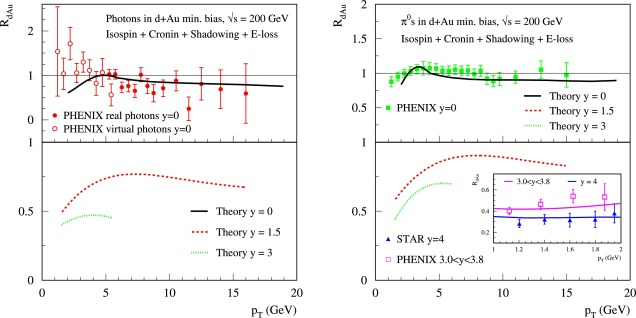
\includegraphics[width=0.99\textwidth]{CNM_cal.jpg}
    \caption{The nuclear modification factor is plotted as a function of transverse momentum for photons (left panel) and \pizero's (right panel) measure with the PHENIX detector.\cite{Kang2012}}
    \label{fig:CNM_calc}
  \end{figure}

  There are additional cold nuclear matter effects, such as anti-shadowing at high bjorken-$x$ and the EMC effect that are not included in the calculation in \cite{Kang2012}. Anti-shadowing is considered to have similar origins as shadowing discussed previously, but is thought to lead to an enhancement at more intermediate $x$ \cite{Brodsky1990a}, approximately above $x\approx_10^{-2}$ \cite{epps16:2017}. The origins of the EMC effect are still not well understood. One model attributes it to mean field modifications, in which close proximity of nucleons may allow quarks in different nucleons to interact directly. Mean-field models predict that all nucleons experience some degree of structure modification, and they are consistent with the observation that the EMC effect increases with nuclear size, scales with local density, and saturates for very large nuclei \cite{Hen2017a}. Another model suggests that rather than all nucleons experiencing some modification, the short-range correlations hypothesis predicts that most nucleons at any one time are unmodified, but some are substantially modified \cite{Norton2003a}.

However, of particular importance for the comparison of this data is EPPS16 nPDF parametrization, which does include these effects. EPPS16 is a nPDF parametrization based on LHC, PHENIX, SLAC, and FNAL, and NMC data \cite{epps16:2017}. The overall $x$-dependant nuclear modification $R_{i}^{A}(x)$ is given by the parametrization:

\begin{equation}
  R_{i}^{A}(x)=\left\{\begin{array}{ll}
      a_{0}+\left(a_{1}+a_{2} x\right)\left[\exp (-x)-\exp \left(-x_{a}\right)\right] & x \leq x_{a} \\
      b_{0}+b_{1} x+b_{2} x^{2}+b_{3} x^{3} & x_{a} \leq x \leq x_{e} \\
      c_{0}+\left(c_{1}-c_{2} x\right)(1-x)^{-\beta} & x_{e} \leq x \leq 1
  \end{array}\right.
\end{equation}

The available collider data is not sufficient to determine the nuclear modification for all parton species separately, so $R_{i}^{A}(x)$ is defined only for valence quarks,  $R_{V}^{A}(x)$, all sea quarks together,  $R_{S}^{A}(x)$, and gluons,  $R_{G}^{A}(x)$. A is the mass number of the nucleus, and  $a_i, b_i, c_i, \beta, x_a,$ and $x_e$ are all A-dependant parameters. 

This parametrization actually already shown in Fig.~\ref{fig:cnm_cartoon}, but is placed here again for convenience.

\begin{figure}[htpb]
  \centering
  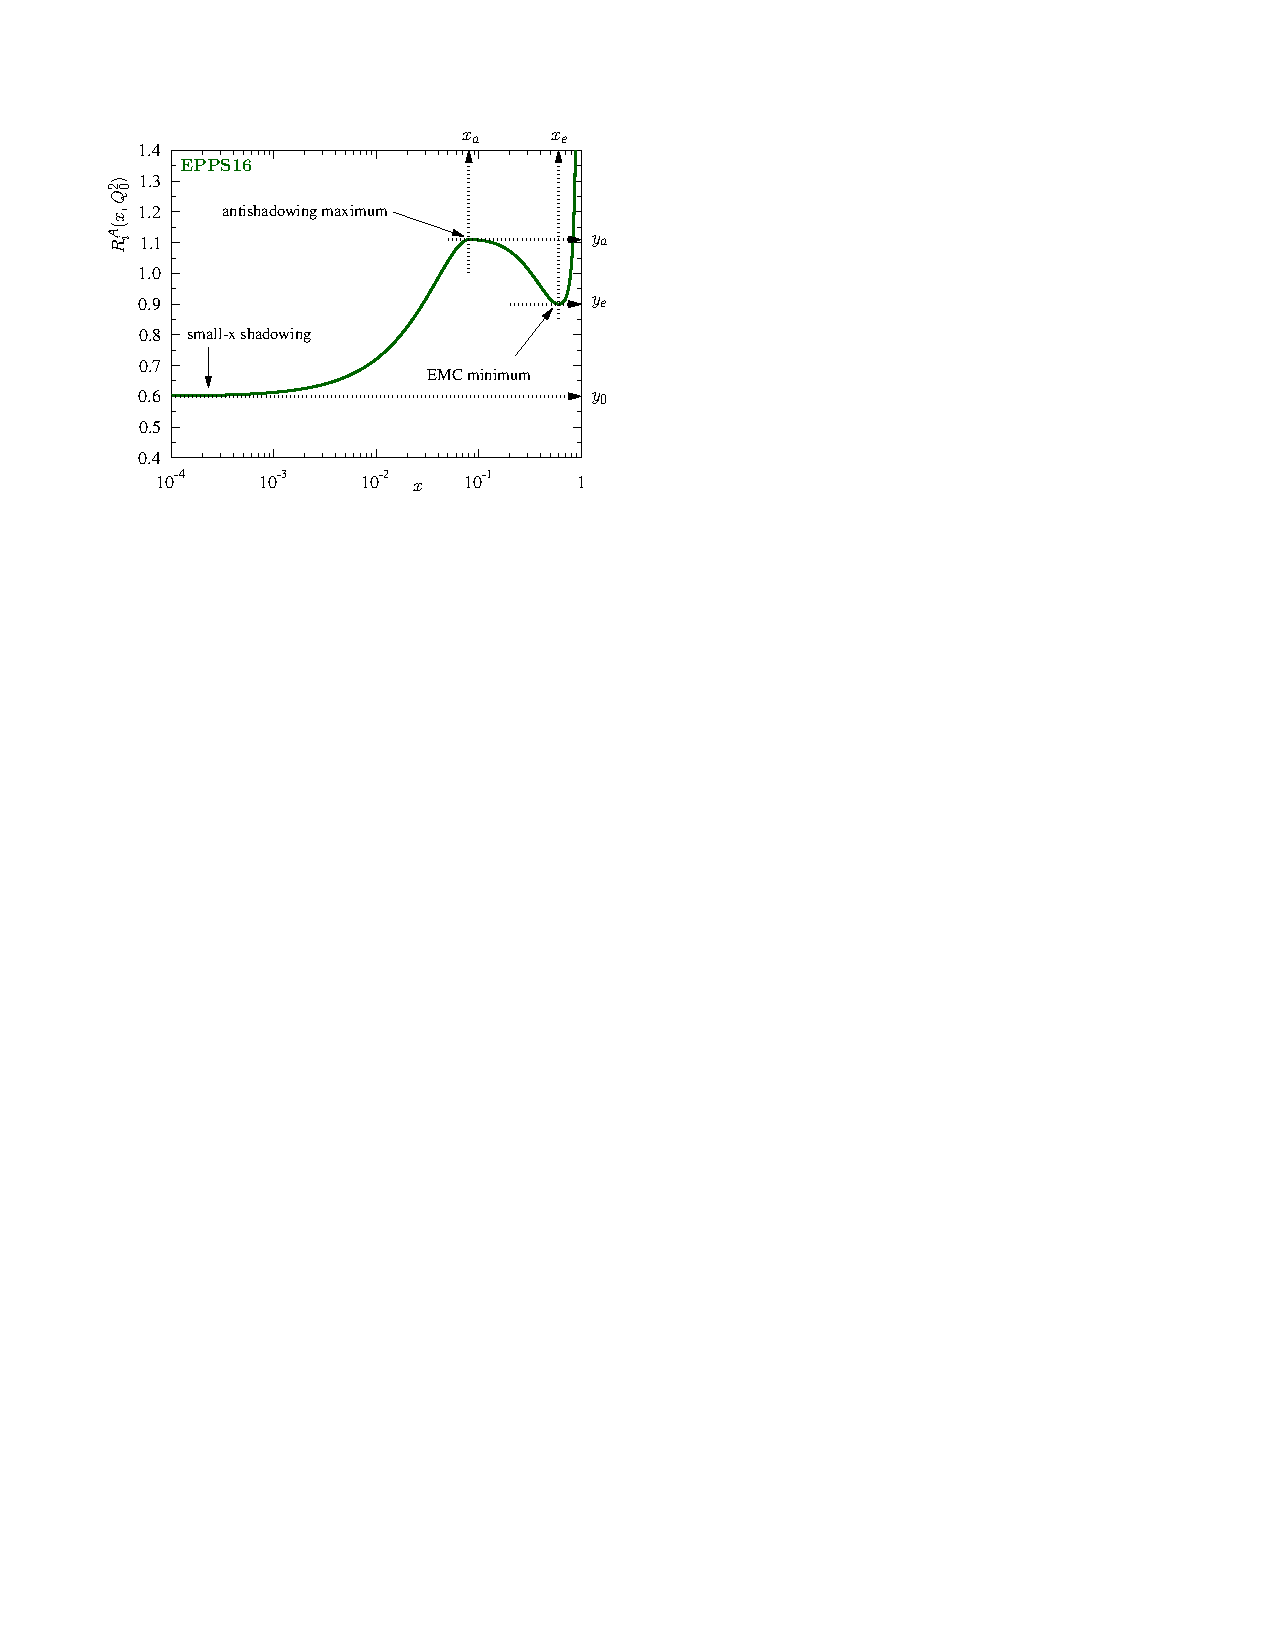
\includegraphics[width=0.7\textwidth]{Introduction/cnm_cartoon}
  \caption{An illustration of the fit function $R_{i}^{A}(x)$ from the EPPS16 parametrization \cite{epps16:2017}.}
  \label{fig:cnm_cartoon_2}
\end{figure}

For the calculation of the $\gammaiso$-hadron spectra in \cite{Xie2021}, the nPDFs from EPPS16 were used. The other key component relevant to the $\gammaiso$-hadron correlations are modifications to the fragmentation function. The calculation in \cite{Xie2021}, uses a vacuum fragmentation function, $D_{h / d}\left(z_{d}, \mu^{2}\right)$, based on the Kniehl-Kramer-Potter parametrization \cite{Kniehl2000}, where $z_d=\pt/p_{\mathrm{T}d}$ is the hadrons momentum fraction when the parton $d$ fragments in vacuum. Vacuum fragmentation is used because the timescale of fragmentation is thought to be sufficiently begins only after the scattered parton is no longer within nucleus. However, a precise estimate of the fragmentation timescale requires a good measurement of $Q^2$ \cite{Sasabe1980}.


% \begin{equation}
%   I_{pA}^{\gamma h}\left(z_{\mathrm{T}}\right)=\frac{D_{p A}^{\gamma h}\left(z_{\mathrm{T}}\right)}{D_{p p}^{\gamma h}\left(z_{\mathrm{T}}\right)}
% \end{equation}

The modification to the yield of associated hadrons in \pPb is quantified as the ratio of yields in \pPb and pp, $I_{pA}^{\gamma h}$. $I_{pA}^{\gamma h}$ is plotted in Fig.~\ref{fig:cnm_Iaa} for the kinematic region most relevant to the measurement detailed in this work.
%For a given  $\zt$, this is given by: 
\begin{figure}[htpb]
  \centering
  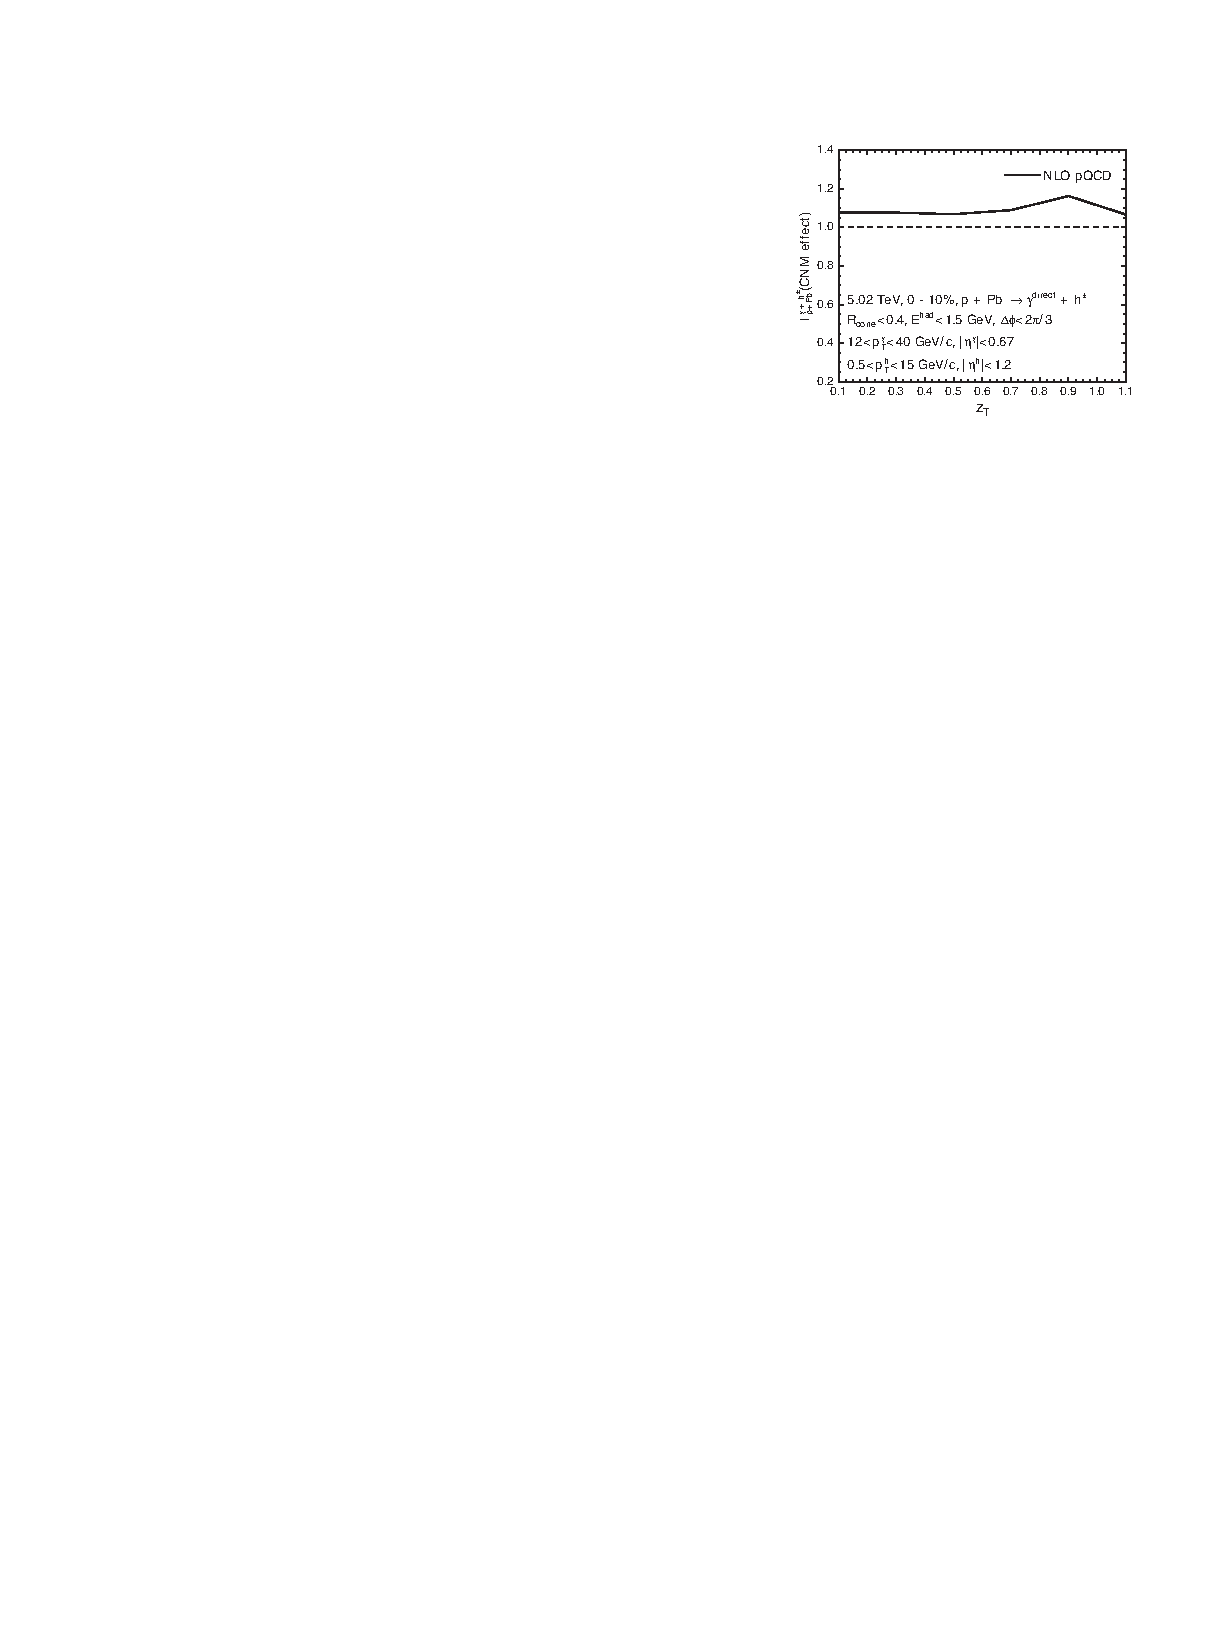
\includegraphics[width=0.7\textwidth]{cnm_Iaa}
  \caption{The modification factor $I_{p P b}^{\gamma h}$ due to CNM effect on $\gamma^{\text {dir}}$-hadron spectra in $p+\mathrm{Pb}$ collisions at $\sqrt{s_{\mathrm{NN}}}=5.02 \mathrm{TeV}$ within $0-10 \%$ centrality \cite{Xie2021}.}
  \label{fig:cnm_Iaa}
\end{figure} 

This calculation is overlayed with the measured data as well as a QGP droplet calculation in Fig.~\ref{fig:FF_model}. It predicts a value of $I_{pA}^{\gamma h}$ above one at higher \zt, meaning there is a higher yield of hadrons in \pPb for that \zt. This is attributed to the anti-shadowing effect from the EPPS16 nPDF. Section \ref{sec:comparison} will discuss in more detail the extent to which our data confirms this prediction. 
% In other words, since the cross section shown in Eq.~\ref{eq:hadron_cross} is factorized into a PDF and fragmentation function component, effects of the nucleus as a medium such as multi-parton interactions must be included in at least on of these terms. For many models of cold nuclear matter effects these properties are modelled in the nPDF. 

%FIXME: talk about how properties of the nucleus as a medium are often modelled to effect the parton before it fragments, and are thus absorbed into the PDF. In this framework, the measurement is in principle sensitive to these effects, as the direct photon should not experience similar effects {reference for the parton effecting part}

%FIXME: talk about CTEQ PDFs in pp briefly, and the specifics of the nPDF parametrization EPPS16. WHAT EFFECTS ARE INCLUDED?


%In the hadronic cross section equation, this is factorized as a separate contribution from the fragmentation function. In the factorized cross section, three scales are usually defined,  
\FloatBarrier
\subsection{Modeling a Droplet of QGP}
The calculation in \cite{Xie2021} models nuclear effects on the $\gamma$-hadron spectra by modeling a small droplet of QGP produced in \pPb~collisions. The model involves the dynamical evolution of the QGP medium that governs the space-time evolution of the local temperature and flow velocity. The droplet dynamics utilize previous studies of jet quenching in A + A collisions, obtained using the (2 + 1) dimensional viscous hydrodynamic model with Monte Carlo-Glauber initial conditions. The scaled jet transport coefficient $\hat{q_0}/T^3_0$, which is the mean $\pt$ transfer between the parton and the medium in each collision, determines the magnitude of energy loss, and is taken from the single inclusive hadron spectra in Au+Au and peripheral Pb+Pb hydrodynamic simulations. 

Importantly, the droplet of QGP should modify the fragmentation function. If $D_{h / d}\left(z_{d}\right)$ is the vacuum fragmentation function, $\tilde{D}_{h / d}\left(z_{d}, \mu^{2}, \Delta E_{d}\right)$ is the hot medium modified fragmentation function, and is related to the vacuum fragmentation function by:

\begin{equation}
  \begin{aligned}
    \tilde{D}_{h / d} &\left(z_{d}, \mu^{2}, \Delta E_{d}\right) \\
    =&\left(1-e^{-\left\langle N_{g}^{d}\right\rangle}\right)\left[\frac{z_{d}^{\prime}}{z_{d}} D_{h / d}\left(z_{d}^{\prime}, \mu^{2}\right)+\left\langle N_{g}^{d}\right\rangle \frac{z_{g}^{\prime}}{z_{d}} D_{h / g}\left(z_{g}^{\prime}, \mu^{2}\right)\right] \\
     &+e^{-\left\langle N_{g}^{d}\right\rangle} D_{h / d}\left(z_{d}, \mu^{2}\right)
  \end{aligned}
\end{equation}
$z_{d}^{\prime}=p_{\mathrm{T}} /\left(p_{\mathrm{T} d}-\Delta E_{d}\right)$ is the momentum fraction of a hadron with transverse momentum \pt~from a parton with initial transverse momentum $p_{\mathrm{T}d}$ that has lost energy $\Delta E_d$ while propagating through the hot medium.  $\langle N_g^d \rangle$ is the average number of radiated gluons and $z_{g}^{\prime}=\left\langle N_{g}^{d}\right\rangle p_{\mathrm{T}} / \Delta E_{d}$ is the momentum fraction of a hadron from a radiated gluon which carries an average energy $\Delta E_{d} /\left\langle N_{g}^{d}\right\rangle$. Lastly, $\left(1-e^{-\left\langle N_{g}^{d}\right\rangle}\right)$ is the probability for a parton to suffer at least one inelastic scattering while propagating through the hot medium. $\Delta E_{d}$ can be calculated by doing an integral over the partons propagation path, $l$, and is detailed in \cite{Wang2002}. $\langle N_g^d \rangle$ is calculated from \cite{Chang2014}.

The expectation of $\gamma$-hadron suppression due to jet quenching in a small droplet of QGP in \pPb~collisions is shown as the orange band in Fig.~\ref{fig:FF_model}. The width of the band represents the uncertainty on the calculation, given by varying the parameters of the caluclation. The leading uncertainty in the calculation arises from varying the QGP formation time, $\tau_0$ between 0.5-1.0fm/$c$. A comparison to the measured data can constrain these parameters, as well as the model in general.

\subsection{Measurements and Models Compared}
\label{sec:comparison}

The comparison between these calculations and this measurement are shown in Fig.~\ref{fig:FF_model}.

\begin{figure}[htpb]
  \centering
  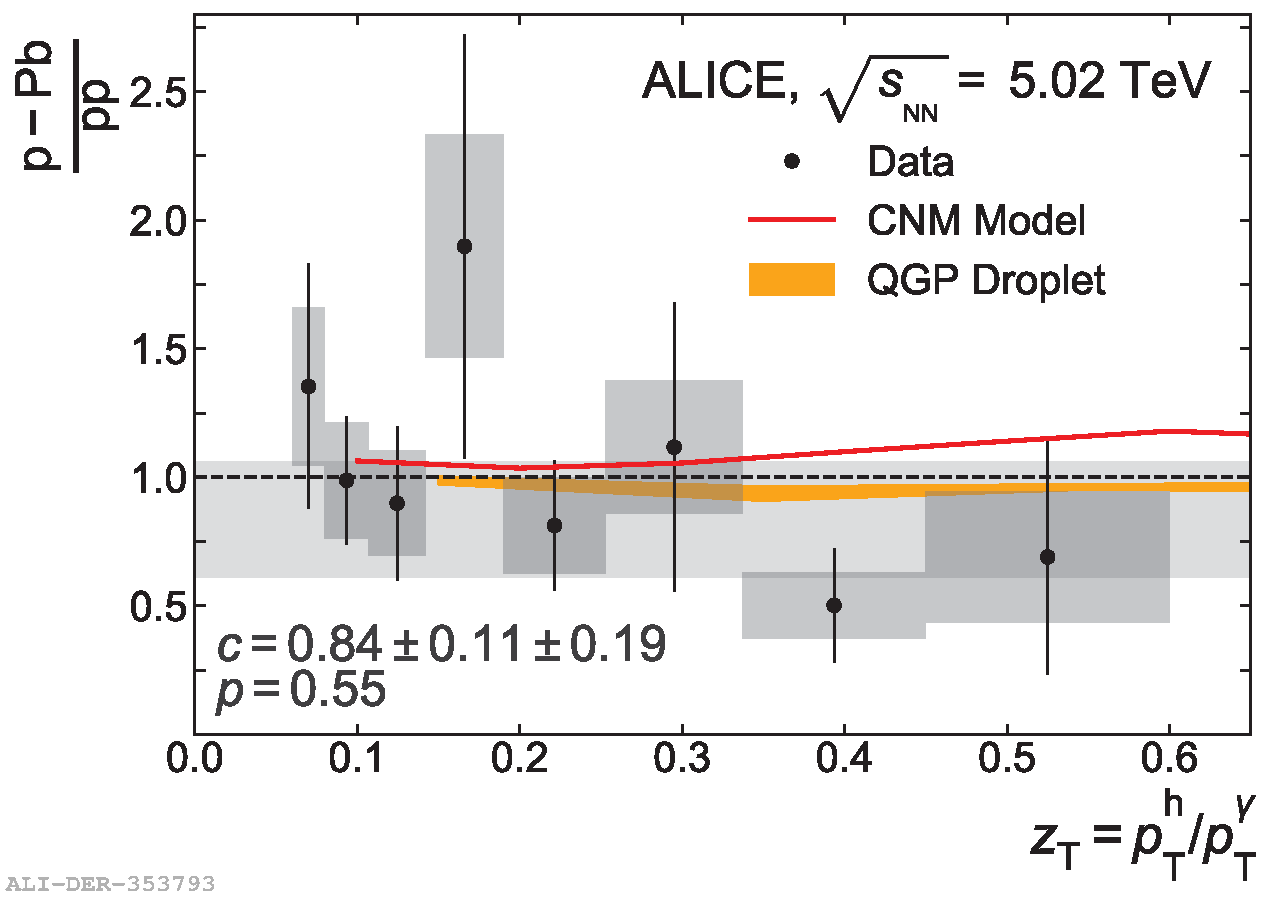
\includegraphics[width=0.8\textwidth]{FF_Model_Comparisons_Ratio.pdf}
  \caption{The ratio of isolated-tagged fragmentation functions for pp and p–Pb data at $\sqrt{s}$ = 5.02 TeV as measured by the ALICE detector.  The ratio is compared to two models from \cite{Xie2021}. The CNM model evolves the partons without parton energy loss, while the quark gluon plasma (QGP) model assumes that a small droplet of QGP is created in p–Pb collisions and applies an energy loss to the partons.}
  \label{fig:FF_model}
\end{figure}
Interestingly, the QGP droplet model predicts that even if a small droplet of QGP were to form, it's effects would be extremely small: it is close to 1.0 in the ratio, well within the statistical and systematic uncertainties in the data. Qualitatively, the calculation being below unity is in line with expectations of energy loss in a small QGP droplet. While the formation of QGP in \pPb~is currently a topic of debate in the field, this model indicates that the modification of the parton fragmentation function in \pPb~is very unlikely to unambiguously reveal its existence. The prediction based on nuclear PDFs tells a very different story. The nuclear modification factor of the PDFs in the CNM model were given by the EPPS16 parametrization \cite{Eskola2017a}. It indicates that if a modification to the parton distribution function were to be observed, it should result in an enhancement at higher \zt, roughly corresponding to the anti-shadowing region at higher Bjorken-$x$ shown in figure \ref{fig:cnm_cartoon_2}. 

The data are consistent with both models. This is not surprising, despite the very different underlying physics that make up the models. The $x_\mathrm{T}$ region of  $0.005 < x_\mathrm{T} < 0.016$ probed in this analysis corresponds to a region in the EPPS16 nPDFs where the modification is close to one; the region is close to the anti-shadowing maximum that corresponds to at most a 10\% effect, and is before the EMC minimum in Fig.~\ref{fig:cnm_cartoon_2}. Larger cold nuclear matter effects are expected to occur at an even lower $x$. A measurement using photon triggers with half the \pt~would probe the nPDFs closer to the shadowing region, where a larger suppression is expected. According to \cite{epps16:2017}, this suppression is expected to be approximately 40\%. However, much higher statistical precision would be needed to measure this with precision. The constant fit to the fragmentation function ratios has an error band of approximately 26\%.

The modifications predicted by the QGP droplet are extremely small for this kinematic range, and would require orders of magnitude more data to distinguish from unity. While flow has been observed in small systems, energy loss or jet suppression has not been observed. The search for energy loss in small systems continues, it at least indicates that hot nuclear matter, if present at all, will have a small effect on the fragmentation function. This means that if a large modification were to observed in \pPb~it is unlikely to be the result of a QGP droplet.

% A common explanation for the observation of flow but no observation energy loss is that the droplet is too small to significantly modify a parton traversing the tiny droplet. 

